\chapter{Nonzero Temperatures}

\section{Introduction}\label{s3.1}
At nonzero temperature, whether electron, phonon, or spin, is interacting with a bath of other particles which have an average energy.
The exact state of all these other particles is not known, since they are fluctuating between different configurations.
All that is know is the temperature, which is related to the mean energy.

\marginnote{
Important knowledge, the expansion
\begin{eqnarray*}
  &&\frac{1}{e^x-1}\\
  &=&\frac{1}{1+x+\frac{x^2}{2!}+\frac{x^3}{3!}+\dots -1}\\
  &=&\frac{1}{x+\frac{x^2}{2!}+\frac{x^3}{3!}+\dots}\\
  &=&\frac{1}{x(1+\frac{x}{2!}+\frac{x^2}{3!}+\dots)}\\
  &\approx&\frac{1}{x(1+\frac{x}{2})}\\
  &\approx&\frac{1}{x}(1-\frac{x}{2}) = \frac{1}{x}-\frac{1}{2}
\end{eqnarray*}
}

When defining the Green's function, one must average over all possible configurations of the system. A possible Green's function for electron is
\begin{eqnarray}
  \frac{\Tr[e^{-\beta H} C_{\bp \sigma}(t) C^\dagger_{\bp \sigma}(t')]}{Tr(e^{-\beta H})}  \label{3.1} \\
  C_{\bp \sigma}(t) = e^{itH}C_{\bp\sigma}e^{-itH}  \label{3.2}
\end{eqnarray}
where $\Tr$ denotes trace and is summation over some complete set of states.

The Matsubara method treats time as a complex temperature, the object is treat $t$ and $\beta$ as the real and imaginary parts of a complex variable, which will require only one $S$-matrix expansion.

The expansion of the series for bosons and fermions give
\begin{eqnarray}
  \eta_F(\xi_\bp) &=& \frac{1}{e^{\beta \xi_\bp}+1} = \frac{1}{2} + \frac{1}{\beta} \sum_{n=-\infty}^\infty \frac{1}{(2n+1)i\pi/\beta -\xi_\bp} \label{3.5} \\
  \eta_B(\omega_\bq) &=& \frac{1}{e^{\beta \omega_\bq}-1} = -\frac{1}{2} + \frac{1}{\beta} \sum_{n=-\infty}^\infty \frac{1}{2ni\pi/\beta -\omega_\bq} \label{3.6}
\end{eqnarray}
\textit{These series can be derived from a theorem which states that any meromorphic function may be expanded as a summation over its poles and residues at those poles}.\footnote{\textcolor{red}{Need to be more clear about this.}}
It is convenient to define the frequencies at the pole
\begin{equation}
  p_n = (2n+1)\pi/\beta,~ ~ ~ ~ \omega_n = 2n\pi/\beta \label{3.7}
\end{equation}

In Matsubara method, time becomes a complex quantity which is usually called $\tau$, where $\tau = it$.
Green's functions are function of $\tau$ with domain
\begin{equation}
  \label{3.10}
  -\beta \leq \tau \leq \beta
\end{equation}
Fourier transform theory states that if a function $f(\tau)$ is defined over such a range, then its Fourier expansion is
\begin{equation}
  \label{3.11}
  f(\tau) = \frac{1}{2}a_0 + \sum_{n=1}^\infty \left[a_n \cos(\frac{n\pi\tau}{\beta}) + b_n \sin(\frac{n\pi\tau}{\beta})\right]
\end{equation}
where
\begin{eqnarray}
  a_n &=& \frac{1}{\beta} \int_{-\beta}^\beta d\tau f(\tau) \cos(\frac{n\pi\tau}{\beta}) \label{3.12} \\
  b_n &=& \frac{1}{\beta} \int_{-\beta}^\beta d\tau f(\tau) \sin(\frac{n\pi\tau}{\beta}) \label{3.13}
\end{eqnarray}
or \textbf{equivalently}. We have
\begin{equation}
  f(i\omega_n) = \frac{1}{2} \beta(a_n + ib_n ) \label{3.14}
\end{equation}
with
\begin{eqnarray}
  f(\tau)&=&\frac{1}{\beta} \sum_{n=-\infty}^\infty e^{-in\pi\tau/\beta} f(i\omega_n) \label{3.15} \\
  f(i\omega_n)&=& \frac{1}{2} \int_{-\beta}^\beta d\tau f(\tau) e^{in\pi\tau/\beta}   \label{3.16}
\end{eqnarray}

\subsection{Boson}
There is still a further simplification can be achieved.
For boson Green's functions have the additional property that
\begin{equation}
  \label{3.17}
  \mathrm{boson:}~ f(\tau) = f(\tau+ \beta),~ ~ -\beta<\tau<0
\end{equation}
Further we have
\begin{eqnarray}
    f(i\omega_n)&=&\int_0^\beta d\tau e^{i\omega_n\tau} f(\tau) \nonumber \\
    f(\tau) &=& \frac{1}{\beta} \sum_n e^{-i\omega_n\tau} f(i\omega_n) \label{3.20} \\
    \omega_n &=& 2n\pi k_BT\nonumber
\end{eqnarray}

\subsection{Fermion}
Similarly, the fermion Green's function will have the property that
\begin{equation}
  \label{3.21}
  \mathrm{fermions:}~ f(\tau) = - f(\tau+ \beta),~ ~ -\beta<\tau<0
\end{equation}
and the result give
\begin{eqnarray}
  f(i\omega_n)&=&\int_0^\beta d\tau e^{i\omega_n\tau}f(\tau) \nonumber \\
  f(\tau)&=&\frac{1}{\beta}\sum_n e^{-i\omega_n\tau}f(i\omega_n) \label(3.23) \\
  \omega_n &=&(2n+1)\pi k_B T \nonumber
\end{eqnarray}

\section{Matsubara Green's functions}\label{s3.2}
The electron Green's function is defined as
\begin{eqnarray}
  \cg(\bp,\tau-\tau') &=& - \langle T_\tau C_{\bp\sigma}(\tau)C^\dagger_{\bp\sigma}(\tau') \rangle  \label{3.24} \\
  \cg(\bp,\tau-\tau')&=& -\Tr \big[e^{-\beta(H-\mu N -\Omega)} T_\tau e^{\tau(H-\mu N)} C_{\bp\sigma}e^{-(\tau-\tau')(H-\mu N)} \nonumber \\
  &\times& C^\dagger_{\bp\sigma} e^{-\tau'(H-\mu N)} \big] \label{3.25} \\
  e^{-\beta \Omega} &=& \Tr(e^{-\beta(H-\mu N)}) \label{3.26}
\end{eqnarray}
The definition is equivalent between \eqref{3.24} and \eqref{3.25}, and it is the thermodynamic average, which is the trace over the complete set of states.
The $\mu$ is the chemical potential and $N$ is the particle number operator.
A grand canonical ensemble is used, where the number of particles is variable.
This many-particle system can be successfully used for one particle in an empty band.
In this case, the analytical continuation is taken as $i\omega_n \to E+ \mu + i\delta$, and the chemical potential will vanish from all expressions.
One is not bothered by the fact that $\beta \mu \ll 0$ in one-particle systems at nonzero temperatures.

In a many-electron system, the chemical potential is retained in the formalism.
The analytical continuation is $i\omega_n \to E+ i\delta$ and energy is measured from the chemical potential.

With some derivation\footnote{P.112~P.114}, we have the Green's functions
\begin{eqnarray}
  \cg(\bp,\tau)&=&-\langle T_\tau C_{\bp\sigma}(\tau) C^\dagger_{\bp\sigma}(0) \rangle \label{3.33}\\
    &=& -\Tr \left[ e^{-\beta (K-\Omega)} T_\tau (e^{\tau K} C_{\bp\sigma} e^{-\tau K} C^\dagger_{\bp\sigma})\right] \label{3.34} \\
  \cg(\bp,i\omega_n) &=& \int_0^\beta d\tau e^{i\omega_n \tau} \cg(\bp,\tau)  \label{3.39} \\
  \cg(\bp,\tau) &=& \frac{1}{\beta} \sum_n e^{-i\omega_n \tau} \cg(\bp,i\omega_n) \label{3.40}
\end{eqnarray}

For noninteracting Green's function, the $\tau$ evolution of the operators is\footnote{Derived from the Baker-Hausdorff theorem
\begin{equation*}
  e^ACe^{-A} = C+ [A,C] + \frac{1}{2!}[A,[A.C]]+\dots
\end{equation*}}
\begin{eqnarray}
  C_{\bp\sigma}(\tau) &=& e^{\tau K_0} C_{\bp\sigma} e^{-\tau K_0} = e^{-\xi_\bp \tau} C_{\bp \sigma } \label{3.44} \\
  C^\dagger_{\bp\sigma}(\tau) &=& e^{\tau K_0} C^\dagger_{\bp\sigma} e^{-\tau K_0} = e^{\xi_\bp \tau} C_{\bp \sigma }^\dagger \label{3.45}
\end{eqnarray}
Then the Green's function is
\begin{equation}
  \cg^0(\bp,\tau)= -e^{-\xi_\bp \tau}[\Theta(\tau)-\eta_F(\xi_\bp)] \label{3.49}
\end{equation}
and
\begin{equation}
  \cg^0(\bp,i\omega_n) = \frac{1}{i\omega_n -\xi_\bp}   \label{3.55}
\end{equation}

The phonon and photon Green's functions are defined in the same fashion,
\begin{eqnarray}
    \cd (\bq,\tau-\tau') &=& - \langle T_\tau \mathbf{A}(\bq,\tau) \mathbf{A}(-\bq,\tau') \rangle \label{3.56} \\
    \mathbf{A}(\bq,\tau) &=& e^{\tau H}(a_\bq+ a^\dagger_{-\bq})e^{-\tau H} \label{3.57}
\end{eqnarray}
and with the relation in \eqref{3.17}, we have
\begin{equation}
  \cd (\bq,\tau) = \cd (\bq, \tau+\beta)~ ~ ~ ~ -\beta<\tau<0 \label{3.63}
\end{equation}

For noninteracting system the Green's function of \textbf{phonons} is
\begin{equation}
  \cd^0(\bq,i\omega_n) = -\frac{2\omega_\bq}{\omega_n^2 + \omega_\bq} \label{3.76}
\end{equation}
Notice that it is almost identical to the zero-temperature case \eqref{2.73}.

The \textbf{photon} Green's function is also identical to its zero-temperature result, except for complex frequencies.
The  fundamental definition is
\begin{eqnarray}
  \cd_{\mu\nu}(\bk,\tau) &=& -\sum_\lambda \langle T_\tau \mathbf{A}_\mu(\bk,\lambda,\tau) \mathbf{A}_\nu(-\bk,\lambda,0)\rangle \label{3.77}\\
  \mathbf{A}_\mu(\bk,\lambda,0) &=& \xi_\mu(\bk,\lambda) (\frac{2\pi}{\omega_\bk})(a_{\bk \lambda}+ a^\dagger_{\bk \lambda}) \label{3.78}\\
  \cd^0_{\mu\nu}(\bk,i\omega_n)&=&-\frac{4\pi(\delta_{\mu\nu}-k_\mu k_\nu/k^2)}{\omega_n^2+\omega_\bk^2} \label{3.79}
\end{eqnarray}

\section{Retarded and advance Green's functions}\label{s3.3}
The retarded and advanced Green's functions were introduced in \ref{s2.9}.
All measurable quantities, such as conductivities or susceptibilities, are actually retarded correlation functions.
The Green's function by Matsubara function can be easily convert to retarded and advanced Green's function.

The retarded Green's functions may be defined for both zero and nonzero temperature.
The retarded Green's function for an electron in state $\bp$ is
\begin{eqnarray}
  G_{ret}(\bp,t-t') &=& G_t(\bp,t-t') - G^<(\bp,t-t')  \\
  &=&-i\Theta(t-t')\langle [C_{\bp\sigma}(t)C^\dagger_{\bp\sigma}(t') + C^\dagger_{\bp\sigma}(t')C_{\bp\sigma}(t)] \rangle \nonumber \\
  &=&-i\Theta(t-t')\Tr \{ e^{-\beta (K-\Omega)} [C_{\bp\sigma}(t) C^\dagger_{\bp\sigma}(t') + C^\dagger_{\bp\sigma}(t')C_{\bp\sigma}(t)]\} \nonumber \label{3.82} \\
  K&=&H-\mu N, ~ ~ ~ ~ C_{\bp\sigma}(t) = e^{iKt}C_{\bp\sigma}e^{-iKt} \label{3.83}
\end{eqnarray}
The Green's function operates only for $t>t'$, which makes it \textbf{causal}.
In the limit that times becomes equal, the anticommutator becomes unity.
The plus sign in the middle of the two terms is an important feature for retarded Green's functions of fermion operators.

For phonons, the retarded Green's function is
\begin{equation}
  D_{ret}(\bq,t-t') = -i\Theta(t-t')\langle A(\bq,t)A(-\bq,t') - A(-\bq,t')A(\bq,t)\rangle \label{3.85}
\end{equation}
The sign in the middle is minus, which corresponding the bosons' commutation relations.

Retarded Green's functions are needed for many types of operators with products of electron or boson operators.
\begin{eqnarray}
  U&=& \sum_{ij}M_{ij}C^\dagger_iC_j \label{3.86}\\
  V&=& \sum_{ijk}M_{ijk}C^\dagger_i C_j C_k \label{3.87}
\end{eqnarray}
The operator $U$ is bilinear in operator $C_i$, this can be regarded as having boson properties.
However, operator $V$ can be regarded as fermion operators.
\begin{eqnarray}
  \bar{U}_{ret}(t-t') &=& -i\Theta(t-t')\langle [U(t)U^\dagger(t') - U^\dagger(t')U(t)] \rangle \label{3.88} \\
  \bar{V}_{ret}(t-t') &=& -i\Theta(t-t')\langle [V(t)V^\dagger(t') + V^\dagger(t')V(t)] \rangle \label{3.89}
\end{eqnarray}
All these retarded function have the Fourier transforms defined by the usual convention:
\begin{equation}
  G_{ret}(\bp,E) = \int_{-\infty}^\infty dt e^{iE(t-t')} G_{ret}(\bp,t-t') \label{3.90}
\end{equation}

The advanced Green's function for each is defined
\begin{eqnarray}
  G_{adv}(\bp,t-t')&=&i\Theta(t-t')\langle [C_{\bp\sigma}(t)C^\dagger_{\bp\sigma}(t') \nonumber \\
  &+& C^\dagger_{\bp\sigma}(t')C_{\bp\sigma}(t)] \rangle \label{3.93} \\
  D_{adv}(\bq,t-t') &=& i\Theta(t-t')\langle A(\bq,t)A(-\bq,t') \nonumber \\
  &-& A(-\bq,t')A(\bq,t)\rangle \label{3.94}
\end{eqnarray}
The only two differences are the sign change in front and that the time domain is now $t'>t$, which is just opposite of that for retarded function.

The advanced functions of energy is defined as usual Fourier transform, and turn out to be \textit{complex conjugate} of the corresponding retarded function.
\begin{equation}
  U_{ret}(\omega) = U_{adv}^\dagger(\omega) \label{3.98}
\end{equation}

The Matsubara function can be changed to a retarded one with just this alteration:
\begin{equation}
  i\omega_n \to \omega + i\delta~ ~ ~ ~ \mathcal{U}(i\omega_n) = U_{ret}(\omega)  \label{3.110}
\end{equation}
This step is called an analytic continuation.
The advanced Green's function can be changed by $i\omega_n \to \omega - i\delta$, since the advanced Green's function is the complex conjugate of the retarded one.

Another quantity is \textbf{spectral function}, it is imaginary part of any retarded function multiplied by 2:
\begin{equation}
  A(\bp,\omega) = -2\Im [G_{ret}(\bp,\omega)]  \label{3.115}
\end{equation}
An expression of this form is called \textbf{Lehmann representation}:
\begin{eqnarray}
  U_{ret}(\omega) &=& \int_{-\infty}^\infty \frac{d\omega'}{2\pi} \frac{A(\omega')}{\omega-\omega'+i\delta} \nonumber \\
  \mathcal{U}(i\omega_n) &=& \int_{-\infty}^\infty \frac{d\omega'}{2\pi} \frac{A(\omega')}{i\omega_n -\omega'} \label{3.118}
\end{eqnarray}

For fermions, the spectral density function is positive, $A(\bp,\omega)>0$.
This positiveness is an important feature, since $A(\bp,\omega)$ is interpreted as a probability function.
\begin{equation}
    1 = \int \frac{d\omega}{2\pi} A(\bp,\omega) \label{3.121}
\end{equation}
For bosons spectral function do not have this property, however, they are always positive for $\omega>0$ and negative for $\omega<0$.

For noninteracting electron the Green's function is
\begin{equation}
  G_{ret}^0 (\bp,E)= \frac{1}{E-\xi_\bp + i\delta} \label{3.129}
\end{equation}
It has one sign $\delta>0$, even in may electron system with a Fermi surface.
The retarded functions do not have $\delta_\bp$ changing sign at the Fermi surface, which makes them easier to use than the zero-temperature Green's function.

The spectral function for the noninteracting Green's function is \footnote{\begin{equation*}
\frac{1}{E-\xi_\bp + i\delta} = \frac{1}{E-\xi_\bp} - \pi i \delta(E-\xi_\bp)
\end{equation*}
check the definition of delta function in \href{https://mathworld.wolfram.com/DeltaFunction.html}{link}}
\begin{equation}
    A^0(\bp, E) = 2\pi \delta(E-\xi_\bp) \label{3.130}
\end{equation}
When $A(\bp,E)$ is computed for interacting systems, there is a broad of the delta function.
This means there is a band of $E$ values for each $\bp$,.
When the electron scatters, it has a nonzero mean free path, and there is some uncertainty in its momentum or energy or both.
So $bp$ and $E$ are treated as separate variables and both are summed over when evaluating physical quantities.

Another quantity to evaluate, for an interacting electron system, is the number of electrons in a momentum state $\bp$, which is
\begin{equation}
  n_\bp = \int \frac{dE}{2\pi} \eta_F(E) A(\bp,E) \label{3.135}
\end{equation}

For phonons, the average number of phonons in a state $\bq$ is
\begin{equation}
  2N_\bq +1  = \langle A^\dagger_\bq A_\bq \rangle = \int \frac{d\omega}{2\pi} \eta_B(\omega)A(\bq,\omega) \label{3.136}
\end{equation}
The noninteracting phonon spectral function is
\begin{equation}
  A^0(\bq,\omega) = 2\pi [\delta(\omega-\omega_\bq) - \delta(\omega+ \omega_\bq)] \label{3.137}
\end{equation}

In later sections the Green's function in Matsubara form have a Dyson form
\begin{eqnarray}
    \cg(\bp,ip_n) &=& \frac{1}{ip_n -\xi_\bp -\Sigma(\bp,ip_n)}     \label{3.138} \\
    \cd (\bq,i\omega_n) &=& \frac{-2\omega_\bq}{\omega_n^2 + \omega_\bq^2 +2\omega_\bq P(\bq,i\omega_n)} \label{3.139}
\end{eqnarray}
Define the retarded self-energies according to \eqref{3.110}
\begin{equation}
  ip_n \to E + i\delta ~ ~ ~ ~ \Sigma(\bp,ip_n) \to \Sigma_{ret}(\bp,E) = \Re \Sigma_{ret} + i \Im \Sigma_{ret}    \label{3.140}
\end{equation}
Consider the retarded Green's function will have a Dyson equation
\begin{equation}
  G_{ret}(\bp,E) = \frac{1}{E+i\delta-\xi_\bp - \Sigma_{ret}(\bp,E)} \label{3.141}
\end{equation}
as derived from \eqref{3.110}.
The spectral function for the electron is rewritten in terms of the retarded self-energy,
\begin{equation}
  A(\bp,E) = \frac{-2 \Im \Sigma_{ret}(\bp,E)}{[E-\xi_\bp - \Re \Sigma_{ret}(\bp,E)]^2 + [\Im\Sigma_{ret}(\bp,E)]^2}  \label{3.142}
\end{equation}

Simple examples to distinguish Matsubara, retarded, and advanced Green's function.
There are some simple functions which have the correct analytical properties.
Considering a self-energy operator has the following functional form,
\begin{equation}
  \Sigma(\bp,Z) = C \ln [f(\bp) -Z] \label{3.143}
\end{equation}
where $Z$ is a complex variable representing the frequency. Take $C$ as a constant and $f(\bp)$ as some function of momentum.
The Matsubara self-energy is evaluated at the points
\begin{equation}
  \Sigma(\bp,ip_n) = C \ln [f(\bp)-ip_n] \label{3.144}
\end{equation}
The analytic continuation $ip_n \to E  \pm i\delta$ to the real axis has the following values.
For retarded function \footnote{
To get this relation
\begin{eqnarray*}
    \Sigma_{ret} &=& C \ln [f(\bp)-E-i\delta]\\
    &=& C \int \frac{dE}{f(\bp)-E-i\delta} + \mathbf{C}
\end{eqnarray*}
}, using $ip_n \to E + i \delta$
\begin{equation}
  \Sigma_{ret}(\bp,E) = C \ln \abs{f(\bp) -E} - i\pi C \Theta[E-f(\bp)] \label{3.145}
\end{equation}
and for advanced
\begin{equation}
  \Sigma_{adv(\bp,E)} = C \ln \abs{f(\bp)-E} + i\pi C \Theta[E-f(\bp)]  \label{3.146}
\end{equation}
These two self-energies differ in the region $E>f(\bp)$, because their imaginary parts have the opposite sign. This difference agrees with the general theorem that
\begin{equation}
  G^*_{ret}(\bp,E) = G_{adv}(\bp,E) \label{3.147}
\end{equation}
and also implies that
\begin{equation}
  \Sigma_{ret}^*(\bp,E) = \Sigma_{adv}(\bp,E) \label{3.148}
\end{equation}
There is a branch cut on the real axis for $E>f(\bp)$. This branch cut just expresses the fact that $\ln(f-Z)$ is not a continuous function of $Z$ across the real axis.

Another example which has the similar analytical properties is
\begin{equation}
  \Sigma(\bp,Z) = C[f(\bp) -Z]^{\frac{1}{2}} \label{3.149}
\end{equation}
This function also has a branch cut for $E>f(\bp)$, with $\Im\Sigma<0$ and $\Im\Sigma>0$.
In fact, a branch cut is a necessary feature whenever $\Im \Sigma \neq 0$, which gives
\begin{equation}
  \Sigma(\bp,E+i\delta) \neq \Sigma(\bp,E-i\delta)  \label{3.150}
\end{equation}
One should be aware that when self-energy functions are evaluated, they are often given by logarithmic or square root function.

When a branch cut occurs and $\Im\Sigma \neq 0$, then the spectral function is given by \eqref{3.142}.
In other regions where there is no branch cut, then take the limit of $\Im\to 0$ and obtain
\begin{equation}
  \lim_{\Im\Sigma=0}A(\bp,E)=2\pi \delta(E-\xi_\bp-\Re\Sigma_{ret}(\bp,E))   \label{3.151}
\end{equation}
Here the spectral function is a delta function, but the real part of the self-energy may be nonzero, so that it affects the spectral function.
Denote by $E(\bp)$ the solution to the equation
\begin{equation}
  E(\bp) -\mu = \xi_\bp + \Re\Sigma(\bp,E(\bp)-\mu) \label{3.152}
\end{equation}
Assume that there is a problem in which \eqref{3.152} is satisfied when $\Im\Sigma=0$.
Then with the properties of delta function, the spectral function is written as
\begin{eqnarray}
  A(\bp,E)&=&2\pi Z(\bp) \delta(E-E(\bp)+\mu) \label{3.154} \\
  Z(\bp)&=&\frac{1}{\abs{1- \frac{\partial}{\partial E} \Sigma_{ret}(\bp,E)}_{E=E(\bp)-\mu}}  \label{3.155}
\end{eqnarray}
The factor $Z(\bp)$ is called \textbf{renormalization factor}.
Because of \eqref{3.121} and $A(\bp,E)>0$, we have $Z(\bp)<1$.
The strength of the delta function peak is always less than or equal to unity.

Equation \eqref{3.152} may be used to define the effective mass. Assume that the noninteracting states are free particles
\begin{equation}
  \xi_\bp = \frac{p^2}{2m} -\mu = \varepsilon_\bp -\mu  \label{3.156}
\end{equation}
Furthermore, assume at low momentum that $E(\bp)$ in \eqref{3.152} varies quadratically wit momentum,
\begin{equation}
  E(\bp) = E_0 + \frac{p^2}{2m^*} +\mathcal{O}(p^4)  \label{3.157}
\end{equation}
The proportionality constant is the inverse effective mass $m^*$
\begin{equation}
  \frac{m}{m^*} = \frac{\partial E(\bp)}{\partial \varepsilon_\bp}  \label{3.158}
\end{equation}
from the definition of \eqref{3.152}, we get
\begin{equation}
  \frac{\partial E(\bp)}{\partial \varepsilon_\bp} = \lim_{\varepsilon_\bp \to 0} \left(1 + \frac{\partial}{\partial \varepsilon_\bp} \Re\Sigma_{ret}(\bp,E) + \left[ \frac{\partial}{\partial E}\Re\Sigma_{ret}(\bp,E) \right] \frac{\partial E(\bp) }{\partial \varepsilon_\bp} \right)  \label{3.159}
\end{equation}
With \eqref{3.158}, the final term is arrived
\begin{equation}
  \frac{m}{m^*} = \lim_{\varepsilon_\bp \to 0} \left[ \frac{1 + (\partial_{\varepsilon_\bp}) \Re \Sigma_{ret}(\bp,E_0-\mu)}{1 - (\partial_{E_0}) \Re \Sigma_{ret}(\bp,E_0-\mu)}\right]  \label{3.160}
\end{equation}
This formula will be frequently to obtain the effective mass from self-energy calculations.

\section{Dyson's Equation} \label{s3.4}
The Matsubara Green's functions are evaluated by the same method of Feynman diagram techniques.
The ideas behind expanding the $S$ matrix are presented, and Dyson's equation is rederived for the Matsubara Green's function in this section.

Consider the case of the electron Green's function:
\begin{eqnarray}
    \cg(\bp,\tau) &=& -e^{\beta \Omega} \Tr\left[ e^{-\beta K} T_\tau (e^{\tau K} C_{\bp}e^{-\tau K} C^\dagger_\bp) \right] \label{3.161} \\
    e^{-\beta \Omega} &=& \Tr(e^{-\beta K}) \label{3.162}
\end{eqnarray}
where we consider the general case
\begin{equation}
    K = K_0 + V = H_0 -\mu N + V \label{3.163}
\end{equation}
where $K_0$ is a problem which can be solved.
The Hamiltonians under consideration usually have the property that they commute with the number operator
\begin{equation}
    \left[H_0,N\right] = \left[H,N\right] = 0 \label{3.166}
\end{equation}
where $H$ and $N$ can be defined in same eigenstates.
Consider the evaluation operations in interaction picture \eqref{2.10}, we have
\begin{equation}
  U(\tau) = e^{\tau K_0} e^{\tau K} ~ ~ ~ U^{-1}(\tau) = e^{\tau K}e^{-\tau K_0}  \label{3.168}
\end{equation}
ant the time dependence of operators
\begin{equation}
  \hat{C}_\bp (\tau ) = e^{\tau K_0}C_\bp e^{-\tau K_0} = e^{-\tau \xi_\bp} C_\bp \label{3.169}
\end{equation}
Then the Green's function in \eqref{3.161}, is written for $\tau>0$ as
\begin{equation}
  \cg(\bp,\tau) = -\frac{\Tr\left[ e^{-\beta K_0} U(\beta) U^{-1}(\tau) \hat{C}_\bp(\tau) U(\tau) C^\dagger_\bp \right]}{\Tr \left[  e^{-\beta K_0} U(\beta)\right]} \label{3.170}
\end{equation}

The operator $U(\tau)$ can be solved in terms of $\tau$-ordered products.
\begin{equation}
  \partial_\tau U(\tau) = -\hat{V}(\tau) U(\tau)  \label{3.173}
\end{equation}
This equation for $U(\tau)$ is given as
\begin{equation}
  U(\tau) = T_\tau \exp\left[- \int_0^\tau d\tau_1 \hat{V}(\tau_1) \right]  \label{3.177}
\end{equation}
Next consider the definition
\begin{equation}
  S(\tau_1,\tau_2) = T_\tau \exp\left[ -\int_{\tau_1}^{\tau_2} d\tau \hat{V}(\tau) \right] \label{3.178}
\end{equation}
as discussed in previous section.
Then with the rearrange terms of \eqref{3.169},
\begin{equation}
  \cg (\bp,\tau) = - \frac{\langle T_\tau S(\beta) \hat{C}_\bp(\tau) \hat{C}^\dagger_\bp \rangle_0}{\langle S(\beta) \rangle_0} \label{3.185}
\end{equation}
This form of the Green's function is similar to the zero-temperature result \eqref{2.50}.

The Green's function is evaluated, at least formally, by expanding the $S$ matrix in the numerator
\begin{eqnarray}
  &&\langle T_\tau S(\beta) \hat{C}_\bp (\tau) \hat{C}^\dagger_\bp \rangle_0  \label{3.186}\\
  &=& \sum_{n=0}^\infty \frac{(-1)^n}{n!} \int_0^\beta d\tau_1 \dots \int_0^\beta d\tau_n  \langle T_\tau \hat{C}_\bp(\tau) \hat{V}(\tau_1) \dots \hat{V}(\tau_n) \hat{C}^\dagger_\bp \rangle_0 \nonumber
\end{eqnarray}
Each of the $n$th terms are evaluated by applying Wick's theorem.
The disconnected diagrams are canceled by the vacuum polarization diagrams which is $e^{-\beta \Omega}$.

Then the Matsubara Green's function can be reduced to an evaluation of all connected different diagrams
\begin{equation}
  \cg(\bp,\tau) = - \sum_{n=0}^\infty (-1)^n \int_0^\beta d\tau_1 \dots \int_0^\beta d\tau_n \langle T_\tau \hat{C}_\bp(\tau)\hat{V}(\tau_1)\dots\hat{V}(\tau_n)\hat{C}_\bp(0) \rangle_0 \label{3.196}
\end{equation}
and the Green's function of energy is found by Fourier transform
\begin{equation}
  \cg(\bp,ip_n) = \int_0^\beta d\tau e^{ip_n\tau}\cg(\bp,\tau) ~ ~ ~ \cg(\bp,\tau) = \frac{1}{\beta} \sum_{p_n} e^{-ip_n\tau} \cg(\bp,ip_n)  \label{3.197}
\end{equation}
The terms in the series \eqref{3.196} yield self-energy diagrams, which may be collected into Dyson equation
\begin{eqnarray}
  \cg(\bp,ip_n) &=& \frac{\cg^0(\bp,ip_n)}{1 - \cg^0(\bp,ip_n) \Sigma(\bp,ip_n)} \label{3.198} \\
  \cd (\bq,i\omega_n) &=& \frac{\cd^0(\bq,i\omega_n)}{1-\cd^0(\bq,i\omega_n) \Pi(\bq,i\omega_n)} \label{3.199}
\end{eqnarray}
The rules for constructing diagrams, are similar in the non-zero temperature cases.

\section{Frequency Summations}\label{s3.5}
When using the Matsubara Green's functions, one must evaluate frequency summations over combinations of unperturbed Green's functions.
The technique for evaluating these summations is discussed for both cases of unperturbed functions and also Green's functions with self-energies.
There is a table of results for combinations which often occur.
\begin{eqnarray}
  -\frac{1}{\beta} \sum_m \cd^0(\bq,i\omega_m)\cg^0(\bp,ip_n+i\omega_m) &=& \frac{N_\bq + \eta_F(\xi_\bp)}{ip_n-\xi_\bp+\omega_\bq} \nonumber \\
  &+& \frac{N_\bq + 1 - \eta_F(\xi_\bp)}{ip_n -\xi_\bp-\omega_\bq} \label{3.216} \\
  \frac{1}{\beta} \sum_n \cg^0(\bp,ip_n) \cg^0(\bk,ip_n+i\omega_m) &=& \frac{\eta_F(\xi_\bp)-\eta_F(\xi_\bk)}{i\omega_m + \xi_\bp -\xi_\bk} \label{3.217} \\
  -\frac{1}{\beta} \sum_n \cg^0(\bp,ip_n) \cg^0(\bk,i\omega_m-ip_n) &=& \frac{1-\eta_F(\xi_\bp) - \eta_F(\xi_\bk)}{i\omega_m -\xi_\bp -\xi_\bk} \label{3.218}\\
  \frac{1}{\beta} \sum_n \cg^0(\bp,ip_n) &=& \eta_F(\xi_\bp)\label{3.219}
\end{eqnarray}

First consider the summation over a boson series, considering \eqref{3.216}, we have this term
\begin{equation}
  S = \frac{1}{\beta} \sum_m \frac{2\omega_\bq}{\omega_m^2+\omega_\bq^2} \frac{1}{ip_n+i\omega_m -\xi_\bp} \label{3.220}
\end{equation}
Denote this equation as
\begin{equation}
  S = -\frac{1}{\beta} \sum_m f(i\omega_m) \label{3.221}
\end{equation}
where $f(i\omega_m)$ is the product of Green's function in \eqref{3.220}. This summation is evaluated by a contour integration. The integral has the form\footnote{This gives $I = \lim_{R\to \infty} \oint \frac{dz}{2\pi i} f(z) \eta_B(z) =0$  if $f(z)$ decay faster than $z^{-1}$.
},
\begin{equation}
  I = \lim_{R\to \infty} \oint \frac{dz}{2\pi i} f(z) \eta_B(z)  \label{3.222}
\end{equation}
The function $\eta_B(z)$ is chosen to generate poles at the points $i\omega_m$ for all even integer $m$ .

The function $f(z)$ is
\begin{equation}
  f(z) = \frac{2\omega_\bq}{z^2-\omega_\bq^2} \frac{1}{ip_n + z - \xi_\bp}  \label{3.224}
\end{equation}
The corresponding poles and residues of integral $I$ in \eqref{3.222} are
\begin{eqnarray}
  z_m &=& i 2\pi m k_B T,~ ~ ~ R_i = \frac{1}{\beta}f(i\omega_m)  \nonumber\\
  z_1 &=& \omega_\bq, ~ ~ ~ ~ R_1 = \frac{N_\bq}{ip_n- \xi_\bp+ \omega_\bq} \nonumber \\
  z_2 &=& -\omega_\bq, ~ ~ ~ R_2 = \frac{N_\bq+1}{ip_n -\xi_\bp-\omega_\bq} \nonumber \\
  z_3 &=& \xi_\bp - ip_n, ~ ~ ~ R_3 = \frac{-2\omega_\bq \eta_F(\xi_\bp)}{(ip_n-\xi_\bp)^2-\omega_\bq^2} \label{3.225}
\end{eqnarray}
Then, $I = \frac{1}{\beta} \sum_m f(i\omega)m + R_1 + R_2 + R_3$, and with \eqref{3.221}.
\begin{equation}
  S = R_1 + R_2 + R_3 \label{3.228}
\end{equation}

The method of evaluating these boson series is quite simple.
To evaluate a series such as \eqref{3.221} on just finds all the simple poles of $f(z)$ which are at points $z_j$ with residues $r_j$ and then
\begin{equation}
  S = \sum_J r_j \eta_B(z_j)  \label{3.229}
\end{equation}
The same procedure is used to evaluate fermion series. Then the summations are of the form
\begin{equation}
  S = - \sum_i r_i \eta_F(z_i)  \label{3.231}
\end{equation}
The minus sign in font occurs because the residue of the fermion $\eta_F$ is $-\frac{1}{\beta}$ and is $\frac{1}{\beta}$ for boson $\eta_B$.
\footnote{
\begin{eqnarray}
    && \Res(\frac{1}{e^{-\beta z_0}-1}) \nonumber \\
    &=& \frac{g(z_0)}{f'(z_0)} \nonumber \\
    &=& \left( -\beta e^{-\beta z_0} \right)^{-1} \nonumber \\
    &=& -\frac{1}{\beta} \nonumber
\end{eqnarray}
}

The last result in \eqref{3.219} is special
\begin{equation}
    \frac{1}{\beta} \sum_n \cg^0 (\bp,ip_n) = \eta_F(\xi_\bp) \nonumber
\end{equation}
Due to the definition, the left side is the Fourier transform of Matsubara Green's function.
The result \eqref{3.129} is just the limit at $\tau \to 0$.
This limit is ambiguous, since a different result is obtained if $\tau=0$ is approached from the positive or negative direction
\begin{eqnarray}
    \cg^0(\bp,\tau= 0^+) &=& - \left[1-\eta_F(\xi_\bp)\right] \label{3.238}\\
    \cg^0(\bp,\tau= 0^-) &=& \eta_F(\xi_\bp)    \label{3.239}
\end{eqnarray}
The result \eqref{3.219} is merely the convention of adopting the limit $\tau = 0^-$.

Consider the example of evaluating the summation \eqref{3.216} except that the Green's function for the electron contains some self-energy terms:
\begin{equation}
    \cg(\bp,ip_n) = \frac{1}{ip_n -\xi_\bp -\Sigma(\bp,ip_n} \label{3.241}
\end{equation}
Letting $ip_n =z$ then the above function has branch cuts along the real $Z$ axis.
These branch cuts arise because of the self-energies $\Sigma(\bp,ip_n)$ as discuss in \ref{s3.3}.
The contour integrals used to evaluate the frequency summations become more complicated because of the branch cut.

The most general possibility when evaluating a summation over Matsubara frequencies is to have all the Green's functions fully dressed.
Then is is common to proceed by first expressing all the Green's functions in the \textbf{Lehmann representation}.
For example, evaluate
\begin{equation}
    S = - \frac{1}{\beta} \sum_m \cd(\bq,i\omega_n) \cg(\bp,ip_n + i\omega_n) \label{3.242}
\end{equation}
Express each Green's function as a frequency integral over its respective spectral function as shown in \eqref{3.118}
\begin{eqnarray}
    \cd (\bq,i\omega_m) &=& \int_{-\infty}^\infty \frac{d\omega}{2\pi} \frac{B(\bq,\omega)}{i\omega_m-\omega}  \label{3.243} \\
    \cg (\bp+\bq,ip_n+i\omega_n) &=& \int_{-\infty}^\infty \frac{d \varepsilon}{2\pi}  \frac{A(\bp+\bq, \varepsilon)}{ip_n + i\omega_m -\varepsilon} \label{3.244}
\end{eqnarray}
and the summation $S$ becomes
\begin{equation}
    S = \int_{-\infty}^\infty \frac{d\omega}{2\pi} B(\bq,\omega) \int_{-\infty}^\infty \frac{d\varepsilon}{2\pi} A(\bp+ \bq,\varepsilon) S_0(ip_n,\omega,\varepsilon) \nonumber
\end{equation}
and
\begin{equation}
    S_0(ip_n,\omega,\varepsilon) = - \frac{1}{\beta} \sum_m \frac{1}{i\omega_m-\omega} \frac{1}{ip_n+i\omega_m-\varepsilon} = \frac{\eta_B(\omega) + \eta_F(\varepsilon)}{ip_n+\omega-\varepsilon}  \nonumber
\end{equation}
The summation $S_0$ is now the easy type which is evaluated using noninteracting Green's functions.
The final result provides for the most general case of fully interacting Green's functions.
In general, any frequency summation can be done by expressing all Green's functions in their \textbf{Lehmann representation}.

\section{Linked Cluster Expansions}\label{s3.6}
Another method for evaluating correlation functions is called the linked cluster method or the cumulant expansion.
It is the method used to evaluating the thermodynamic potential $\Omega$.
However, the method has also been applied to evaluating Green's function of time for a few problems as an alternative to Dyson equation approach.

\subsection{Thermodynamic Potential}
The thermodynamic potential is found from the equation
\begin{equation}
    e^{-\beta \Omega} = \Tr (e^{-\beta K} ) = \Tr[e^{-\beta K_0}S(\beta)]   \label{3.251}
\end{equation}
This quantity is useful to evaluate by itself, for example, if $N_e$ is the number of electrons
\begin{eqnarray}
    - \frac{\partial \Omega}{\beta \partial \mu} &=& \langle N_e \rangle  \label{3.252} \\
    \frac{\partial (\beta \Omega)}{\partial \beta} &=& \langle K \rangle = U - \mu \bar{N_e} = \Omega + TS \label{3.253} \\
    m \frac{\partial \Omega}{\partial m} &=& \langle \sum_i \frac{p_i^2}{2m} \rangle = \sum_\bp n_\bp \frac{p^2}{2m}     \label{3.254}
\end{eqnarray}
where $n_\bp$ is the number of electrons with momentum $\bp$ in \eqref{3.135}.

For an interacting system
\begin{equation}
    K = K_0 + V \label{3.256}
\end{equation}
For a system of electrons and phonons,
\begin{equation}
    K_0 = \sum_{\bp,\sigma} \xi_\bp C^\dagger_{\bp\sigma} C_{\bp\sigma} + \sum_\bq \omega_\bq (a^\dagger_\bq a_\bq + \frac{1}{2} )  \label{3.258}
\end{equation}
the trace is simple since the noninteracting eigenstates can be used to expand the trace eigenstates
\begin{equation}
    e^{-\beta \Omega_0} = \Pi_\bp (1 + e^{-\beta \xi_\bp})^2 \Pi_\bq ( \frac{e^{-\beta \omega_\bq/2}}{1 - e^{-\beta \omega_\bq}} )  \label{3.259}
\end{equation}
The logarithm of both sides of this equation
\begin{equation}
    \beta \Omega_0 = -2 \sum_\bp \ln (1 + e^{-\beta \xi_\bp}) + \sum_\bq [ \ln(1- e^{-\beta \omega_\bq}) + \frac{1}{2} \beta \omega_\bq]
\end{equation}
The factor of $2$ in front of electron is the spin degeneracy.
The last term on the right is zero-point energy of phonons.
Change the summations to integrals a factor appears of the volume $v$.
The thermodynamic potential is proportional to the volume of the system.
This result is also apparent from \eqref{3.252} to \eqref{3.254}, since the right-hand side in each case is proportional to the volume or to the number of particles.

To calculate \eqref{3.251} including $S(\beta)$.
The interaction $V$ will add some correction terms to $\Omega_0$ which changes it into $\Omega$.
The method of evaluating this correlation function is by the $S$-matrix expansion
\begin{equation}
    e^{-\beta \Omega} = e^{-\beta \Omega_0} \sum_{n=0}^\infty \frac{(-1)^n}{n!} \int_0^\beta d\tau_1 \dots \int_0^\beta d\tau_n \langle T_\tau \hat{V}(\tau_1) \dots \hat{V}(\tau_n) \rangle_0  \label{3.195}
\end{equation}
In evaluating the right-hand side, all diagrams are included, whether connected or disconnected, since there is no other series at hand to cancel the disconnected diagrams.
The way of doing this expansion is the linked cluster expansion.

The way to do this is stated here.
First, introduce the parameter $\lambda$, to keep track of the number of times the potential occurs in each term in the $S$ matrix.
The $S$-matrix expansion in \eqref{3.195} may be written as
\begin{eqnarray}
    e^{-\beta \Omega} &=& e^{-\beta \Omega_0} \sum_{n=0}^\infty \lambda^n W_n   \label{3.262} \\
    W_n &=& \frac{(-1)^n}{n!} \int_0^\beta d\tau_1 \dots \int_0^\beta d\tau_n \langle T_\tau \hat{V}(\tau_1) \dots \hat{V}(\tau_n) \rangle_0    \label{3.263}
\end{eqnarray}
The basic linked cluster theorem is that this series can be resummed into
\begin{eqnarray}
    e^{-\beta \Omega} &=& \exp \left( -\beta \Omega_0 + \sum_{l=1}^\infty \lambda^l U_l \right) \label{3.264} \\
    U_l &=& \frac{(-1)^l}{l} \int_0^\beta d\tau_1 \dots \int_0^\beta d\tau_l \langle T_\tau \hat{V}(\tau_1) \dots \hat{V}(\tau_l) \rangle_0 \label{3.265}
\end{eqnarray}
where $U_l$ contains just different, connected diagrams: The thermodynamic potential is obtained by setting $\lambda=1$ in \eqref{3.264},
\begin{equation}
    \Omega = \Omega_0 - \frac{1}{\beta} \sum_{l=1}^\infty U_l  \label{3.266}
\end{equation}
\textbf{The basic theorem is that the thermodynamic potential is the summation of the different connected diagrams.}
With some discussion discussed in the book\footnote{P144, Mahan}, we have the identity
\begin{equation}
    U_l = \frac{(-1)^k}{l!} \int_0^\beta d \tau_1 \dots \int_0^\beta d \tau_l \langle T_\tau \hat{V}(\tau_1) \dots \hat{V}(\tau_l) \rangle_{connected}  \label{3.274}
\end{equation}
In terms of the Green's functions, we have
\begin{equation}
    U_l = \frac{1}{l!} \int_0^\beta d \tau_1 \dots \int_0^\beta d \tau_l \cg^)(\bp_1, \tau_1 - \tau_j) \cg^0(\bp_2, \tau_2 - \tau_k) \dots  \label{3.275}
\end{equation}

In prior section, the Green's function $\cg(\bp,\tau)$ was evaluated by a similar expansion technique.
There the connected diagrams obeyed the counting rules that
\begin{equation}
    \frac{1}{l!} \langle T_\tau \hat{C}_{\bp\sigma}(\tau) \hat{V}(\tau_1) \dots \hat{V}(\tau_l) \hat{C}^\dagger_{\bp\sigma}(0) \rangle_{connected} = \langle T_\tau \hat{C}_{\bp\sigma}(\tau) \hat{V}(\tau_1) \dots \hat{V}(\tau_l) \hat{C}^\dagger_{\bp\sigma}(0) \rangle_{different~connected}    \label{3.276}
\end{equation}
Here there are $l\! $ arrangements which are identical.
In the linked cluster method there are only $(l-1)! $.

Next consider the evaluation of the thermodynamic potential.
It is obtained by evaluating the series of terms in\eqref{3.266}.
An example is shown here in Fig.\ref{fig:3.9} for the electron-phonon interaction.
\begin{figure}[h]
    \centering
    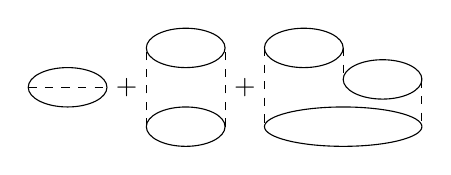
\begin{tikzpicture}
        \draw (0,0) ellipse (0.5 and 0.25);
        \draw [dashed] (-0.5,0)--(0.5,0);
        \node at (0.75,0) {$+$};
        \draw (1.5,0.5) ellipse (0.5 and 0.25);
        \draw (1.5,-0.5) ellipse (0.5 and 0.25);
        \draw [dashed] (1,-0.5)--(1,0.5);
        \draw [dashed] (2.,-0.5)--(2.,0.5);
        \node at (2.25,0) {$+$};
        \draw (3.,0.5) ellipse (0.5 and 0.25);
        \draw (4.,0.1) ellipse (0.5 and 0.25);
        \draw (3.5,-0.5) ellipse (1 and 0.25);
        \draw [dashed] (2.5,0.5)--(2.5,-0.5);
        \draw [dashed] (4.5,0.1)--(4.5,-0.5);
        \draw [dashed] (3.5,0.5)--(3.5,0.1);
    \end{tikzpicture}
    \caption{Link cluster diagram.}%
    \label{fig:3.9}
\end{figure}
They can be summed to give an approximate simple answer.
The rules for constructing diagrams for the terms in the thermodynamic potential are similar to those in Sec~\ref{s3.4}.
One follows all those rules and then multiplies the result by $\frac{\beta}{l}$.
The $ \frac{1}{l} $ factor is just the one which occurs in \eqref{3.265}.
For the first bubble in Fig.~\ref{fig:3.9},
\begin{equation}
    U_2 = \frac{\beta}{2} \frac{\lambda^2}{\beta} \sum_{\bq,iq_n} M^2_\bq \cd^0(\bq,iq_n) P^1(\bq,iq_n)   \label{3.280}
\end{equation}
where the polarization diagram $P^1(\bq,iq_n)$ is for the single bubble, which was already evaluated
\begin{equation}
    P^1(\bq,iq_n) = \frac{2}{\beta V} \sum_{\bp,ip_m} \cg^0(\bp,ip_m) \cg^0(\bp+\bq,ip_m+iq_n)  \label{3.281}
\end{equation}
The second term in Fig.~\ref{fig:3.9} has two bubbles connected by two phonon lines. Using the rules for constructing diagrams gives
\begin{equation}
    U_4 = \frac{\beta}{4} \frac{\lambda^4}{\beta} \sum_{\bq,iq_m} \left[ M_\bq^2 \cd^0(\bq,iq_n) \mathcal{P}^1(\bq,iq+n) \right]^2  \label{3.282}
\end{equation}
Momentum and frequency conservation requires both phonons to have the same variables $(\bq,iq_n)$ and both polarization diagrams are also just functions of combination.
The term with $n$ bubbles and $n$ phonon lines is
\begin{equation}
    U_{2n} = \frac{\beta}{2n} \frac{\lambda^{2n}}{\beta} \sum_{\bq,iq_n} \left[ M^2_\bq \cd^0(\bq,iq_n) \mathcal{P}^1(\bq,iq_n) \right]^n   \label{3.283}
\end{equation}
It is simple to sum the series
\begin{equation}
    \Omega - \Omega_0 = - \frac{1}{\beta} \sum_{n=1}^\infty U_{2n} = \frac{1}{2\beta} \sum_{\bq,iq_n} \ln \left[ 1-\lambda^2 M^2_\bq \cd^0(\bq,iq_n) \mathcal{P}^1(\bq,iq_n)  \right]        \label{3.284}
\end{equation}
This is the correction to the thermodynamic potential.
The right-hand side is proportional to the volume $V$, as is obvious when the summation over $\bq$ is changed to an integration.
The argument of the logarithm is not dependent on $V$, and $V$ enters only by multiplying the result.

The answer in \eqref{3.284} is a logarithm.
The summation over $iq_n$ needs to the evaluated.
A standard trick for eliminating the logarithm, although it does not eliminate it but just disguises it.
Treat $\eta = \lambda^2$ as a variable of integration
\begin{eqnarray}
    &&\int_0^{\lambda^2} d\eta \frac{\Lambda}{1 - \eta\Lambda} = -\ln \left[1 -\lambda^2 \Lambda \right] \label{3.286} \\
    && \Lambda = M^2_\bq \cd^0(\bq,iq_n) \mathcal{P}^1(\bq,iq_n) \label{3.287}
\end{eqnarray}
Then for $\lambda =1$
\begin{equation}
    \Omega- \Omega_0 = - \frac{V}{2\beta} \sum_{iq_n} \int \frac{d^3 q}{(2\pi)^3} \int_0^1 d\eta \frac{M_\bq^2 \cd^0 \mathcal{P}^1}{1 - \eta M^2_\bq \cd^0 \mathcal{P}^1} \label{3.288}
\end{equation}
The logarithm has been eliminated, but now the right-hand side must be evaluated for each value of $\eta$ and then the integral is taken over $\eta$.
\textit{Since $\eta$ enters in the same way as a coupling constant}, this step is called a \textbf{coupling constant integration}.
The integration can be taken outside of the summation over $iq_n$, which makes this summation easier in some case.

Further, define the phonon self-energy as
\begin{equation}
    \pi^1(\eta,\bq,iq_n) = \eta M^2_\bq \mathcal{P}^1(\bq,iq_n) \label{3.289}
\end{equation}
where the coupling constant $\eta$ is included in the definition.
The superscript indicates that this expression is an approximate self-energy, which only includes the single-electron bubble.
The phonon Green's function is
\begin{equation}
    \cd^1(\eta,\bq,iq_n) = \frac{\cd^0}{1-\cd^0 \pi^1}  \label{3.290}
\end{equation}
The Green's function is also a function of the coupling constant strength $\eta$.
Equation \eqref{3.288} is rewritten as
\begin{equation}
    \Omega - \Omega_0 = - \frac{V}{2\beta} \sum_{iq_n} \int \frac{d^3q}{(2\pi)^3} \int_0^1 \frac{d \eta}{\eta} \pi^{(1)}(\eta,\bq,iq_n) \cd^{(1)}(\eta,\bq,iq_n)    \label{3.291}
\end{equation}
This expression is an approximation to $\Omega$ since it employs an approximate self-energy $\pi^{(1)}$.
According the \cite{abrikosov1963methods}, the exact correction to the themodynamic potential from electron-phonon interactions is
\begin{equation}
    \Omega - \Omega_0 = - \frac{V}{2\beta} \sum_{iq_n} \int \frac{d^3q}{(2\pi)^3} \int_0^1 \frac{d \eta}{\eta} \pi(\eta,\bq,iq_n) \cd(\eta,\bq,iq_n)    \label{3.292}
\end{equation}
where $\pi(\eta,\bq,iq_n)$ is the exact phonon self-energy and $\cd(\eta,\bq,iq_n)$ is the exact phonon Green's function evaluated withe excat self-energy.
\begin{figure}[ht]
    \centering
    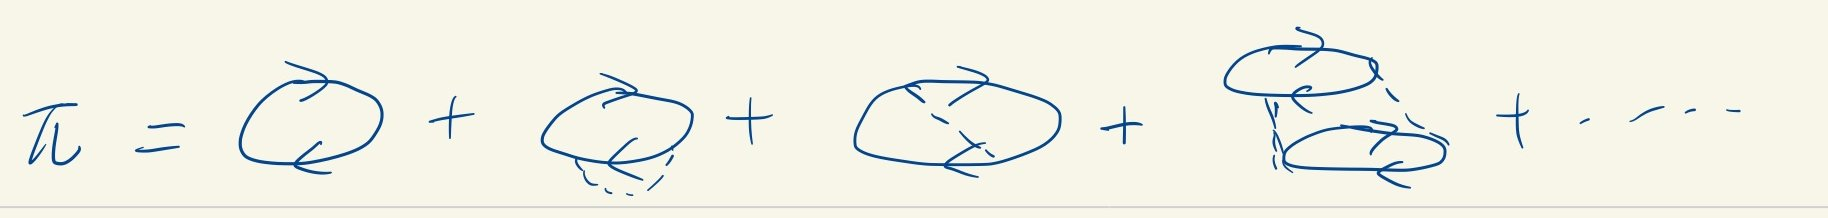
\includegraphics[width=0.8\linewidth]{fig/fig3-10.jpg}
    \caption{The exact phonon self-energy $\pi(\eta,\bq,iq_n)$ is the summation of this infinite number of diagrams. There are bubbles with internal phonon lines and also several bubbles connected by more then on phonon line.}%
    \label{fig:3.10}
\end{figure}

If electron-electron interactions are included, then the phonon self-energy can also contain internal Coulomb interactions, etc.
The effect of Coulomb interaction on the thermodynamic potential should also be included.
THe general theorem \eqref{3.265} and \eqref{3.266} is true for all interactions: Coulomb, phonon, or others.

It is possible to combine the effects of phonons and Coulomb interaction in a simple way.
Consider electrons interacting by either or both interactions, and then the single-bubble diagram appears twices.
The two electron vertives can be connected by a single Coulomb line or a single phonon line. The sum of these contributions is

It is possible to combine the effects of phonons and Coulomb interaction in a simple way.
Consider electrons interacting by either or both interactions, and then the single-bubble diagram appears twices.
The two electron vertives can be connected by a single Coulomb line or a single phonon line. The sum of these contributions is
\begin{equation}
    U_2 = \frac{\eta}{2} \sum_{\bq,iq_n} \mathcal{P}^{(1)}(\bq,iq_n) \left[ M_\bq^2 \cd^{(0)}(\bq,iq_n)\right] \label{3.293}
\end{equation}
By introduce a combined interaction propagator, Coulomb plus phonon, which is
\begin{equation}
    W^{(0)} (\bq,iq_n) = v_q + M_\bq^2 \cd^{(0)}(\bq,iq_n)  \label{3.295}
\end{equation}
with the Dyson equation
\begin{equation}
    W(\bq,iq_n) = \frac{W^{(0)}(\bq,iq_n)}{1-W^{(0)}(\bq,iq_n)\mathcal{P}^{(1)}}     \label{3.296}
\end{equation}
The generalization of \eqref{3.292} to include both Coulomb and phonon effect is
\begin{eqnarray}
    \Omega- \Omega_0 &=& - \frac{V}{2\beta} \sum_{iq_n} \int \frac{d^3 q}{(2\pi)^3} \int_0^1 \frac{d\eta}{\eta} \pi(\eta,\bq,iq_n) W(\eta,\bq,iq_n) \nonumber\\
    &+& \frac{\eta}{2} \int \frac{d^3q}{(2\pi)^3} v_q \label{3.297}
\end{eqnarray}
The first term contains the Coulomb self-energy of an electron interacting with itself, and this unwanted contribution is substracted out in the second term.
The expression \eqref{3.292} is in the expression of phonon self-energies.
It is also posibble to use electron self-energy, considering \eqref{3.272}
\begin{equation}
    U_2 = \frac{\lambda}{2} \sum_{ip_n,\bp,\sigma} cg^{(0)}(\bp,ip_n) \Sigma^{(1)}(\bp,ip_n)    \label{3.298}
\end{equation}
where $\Sigma^{(1)}$ is the electron self-energy from one-phonon processes, which gives
\begin{equation}
    \Sigma^{(1)}(\bp,ip_n) = \frac{1}{\beta V} \sum_{\bq,iq_m} M^2_\bq \cg^{(0)}(\bq+\bp,ip_n+iq_m) \cd^{(0)}(\bq,iq_m)
\end{equation}

These formulas are often used to calculate the ground state energy in the limit of $T\to0$.
There are two limits which are taken: $V\to\infty$ and $T\to0$.
In studying the electron gas, to get the right answer one needs to take the limit of $V\to\infty$ first.
The reverse order omits important terms,
\begin{equation}
    \beta \eta_F(\xi_\bp) \left[ 1-\eta_f(\xi_\bp)\right]   \label{3.300}
\end{equation}
If $V\neq \infty$, then all levels are discrete in finite volume and as $T\to0$ these terms give zero since either $\eta_F$ or $\left[1-\eta_F\right]$ is zero.
However, if one first takes $V\to\infty$, so that the levels are continuous, then the limit $T\to 0$ gives
\begin{equation}
    \lim_{T\to0} \beta eta_F(\xi_\bp)\left[1 -\eta_F(\xi_\bq)\right] = \lim_{T\to0} \frac{d}{d \xi_\bp} \left[ -\eta_F(\xi_\bp) \right] = \delta(\xi_\bp)   \label{3.301}
\end{equation}
There are many terms of this kind in perurbation expansion for the ground state energy of the electron gas.
They are called \textbf{dangerous diagrams}.

Here we show a simple example of evaluating the thermodynamic potntial.
Assume that the onley effect of the phonon self-energy is to change the unperturbed frequencies $\omega_\bq^2$ to a new set of renormalized frequencies $\Omega^2_\bq$.
Since the Green's function is
\begin{equation}
    \cd = \frac{2\omega_\bq}{(i\omega_n)^2 - \omega_\bq^2 - 2\omega_\bq \pi(\bp,i\omega_n)} = \frac{2\omega_\bq}{(i\omega_n)^2 - \Omega_\bq^2} \label{3.302}
\end{equation}
This form for $\cd$ can be accomplished choosing
\begin{equation}
    2\omega_\bq \pi(\eta,\bp,i\omega_n) = \eta(\Omega_\bq^2 - \omega_\bq^2)     \label{3.303}
\end{equation}
The choice \eqref{3.303} is not the only possible one to renormalize the frequencies.
It is the choice one gets by assuming that the change from $\omega_\bq$ to $\Omega_\bq$ is accomplished by the one-bubble polarization diagram given in \eqref{3.289}.
Then the coupling constant $\eta$ enters as just a mulitplicative factor, as shown in \eqref{3.303}.
If further self-energy diagrams are needed to get a good phonon $\pi$, then $\eta$ would enter in a more complicated fashion.
But usually the single-bubble approximation is often adequate.

Consider the \eqref{3.292}, the expression to be evaluated is
\begin{equation}
    \Omega-\Omega_0 = - \frac{1}{2\beta} \sum_{\bq,iq_n} \int_0^1 d\eta \frac{\Omega_\bq^2 -\omega_\bq^2}{(iq+n)^2 -\omega_\bq^2 -\eta(\Omega_\bq^2-\omega_\bq^2)}  \label{3.304}
\end{equation}
Introduce the frequency
\begin{equation}
    \Omega_\eta^2 = \omega^2_\bq + \eta(\Omega_\bq^2 - \omega_\bq^2)    \label{3.305}
\end{equation}
The summation over Matsubara frequencies can be done easily since,
\begin{equation}
    \frac{1}{\beta} \sum_{iq_n} \frac{1}{(iq_n)^2 - \Omega_\eta^2} = \frac{1}{2\Omega_\eta} \cd_\eta(\tau=0) = - \frac{1}{2\Omega_\eta} \left[ 2\eta_B(\Omega_\eta)+1 \right]   \label{3.306}
\end{equation}
Then the evaluaion of \eqref{3.304} is just the coupling constant integral,
\begin{eqnarray}
    &&\Omega-\Omega_0 = \frac{1}{2} \sum_\bq (\Omega_\bq^2 - \omega_\bq^2) \int_0^1 \frac{d\eta}{2\Omega_\eta} \left(1 + \frac{2}{e^{\beta\Omega_\eta}-1}\right) \nonumber \\
    &&= \frac{1}{2} \sum_\bq \left[ \Omega_\eta + \frac{2}{\beta} \ln \left(1-e^{-\beta\Omega_\eta} \right) \right]^{\eta=1}_{\eta=0} \nonumber \\
    &&= \sum_\bq \left[ \frac{1}{2} \left( \Omega_\bq - \omega_\bq \right) + \frac{1}{\beta} \ln \left( \frac{1-\exp (-\beta \Omega_\bq) }{1- \exp(-\beta \omega_\bq)} \right)\right] \label{3.310}
\end{eqnarray}
The right-hand side is the thermodynamic potential from the phonons at the new frequency $\Omega_\bq$ minus the contribution from the phonons at the old frequencies $\omega_\bq$.
When this result is combined with \eqref{3.260} for $\Omega_0$, the terms with $\omega_\bq$ all cancel. THe final answer is
\begin{equation}
    \Omega = -\frac{2V}{\beta} \int \frac{d^3 p}{(2\pi)^3} \ln \left( 1 + e^{-\beta \xi_\bp} \right) + \frac{V}{\beta} \int \frac{d^3 q}{(2\pi)^2} \left[ \frac{1}{2} \beta \Omega_\bq + \ln\left( 1-e^{-\beta \Omega_\bq}  \right) \right]      \label{3.311}
\end{equation}

\section{Real-Time Green's Function} \label{s.3.7}
For six different Green's function of time, the retarded and advanced function have been discussed at nonzero temperature.
The usefulness of the real-time functions is in the treatment of non-equilibrium phenomena.

The Matsubara method is unsuitable for the non-equilibrium since there is no thermodynamic basis for a system out of equilibrium.
The entire Matsubara method is based on temperature, and no method has been found so far for extending it to nonequilibrium processes.

The real-time functions at nonzero temperature have formal definitions very similar to those at zero temperature.
Comparing with \eqref{2.144}, the Green's functions for electrons of momentum $\bp$ are
\begin{eqnarray}
    \cg^<(\bp,t_1,t_2) &=& i\langle C^\dagger_{\bp\sigma}(t_2) C_{\bp\sigma}(t_1) \rangle \nonumber \\
    \cg^>(\bp,t_1,t_2) &=& -i\langle C_{\bp\sigma}(t_1) C_{\bp\sigma}^\dagger(t_2) \rangle \nonumber \\
    \cg_t(\bp,t_1,t_2) &=& \Theta(t_1-t_2) \cg^>(\bp,t_1,t_2) + \Theta(t_2-t_1) \cg^<(\bp,t_1,t_2) \nonumber \\
    \cg_{\bar{t}}(\bp,t_1,t_2) &=& \Theta(t_2-t_1) \cg^>(\bp,t_1,t_2) + \Theta(t_1-t_2) \cg^<(\bp,t_1,t_2)  \label{3.322}
\end{eqnarray}
These definitions appear to be identical to those at zero temperature.
The definition of $\langle \dots \rangle$ have different meanings, depending on the circumstance:
\begin{itemize}
    \item At zero temperature, and in equilibrium, $\langle \dots \rangle$ denote the ground state of the interacting system
    \item At nonzero temperature, and in equilibrium, the brackets denote the thermodynamic average as in \eqref{3.25} and \eqref{3.82}
    \item When not in equilibrium, the brackets denote an average over the accessible phase space. However, the available phase space depends upon the recent history of the system, and kinetic constrains such as energy conservation. The meaning of brackets is poorly understood for system out of equilibrium.
\end{itemize}
Note in \eqref{3.322} that the Green's functions are not expressed on the difference of the time.
This is only true for equilibrium system.

In thermal equilibrium, the real-time functions each have a simple relation to the retarded function.
Using the state $\ket{n}$ and $\ket{m}$, which are exact eigenstates of the Hamiltonian, we have\footnote{P120 and P155 in Mahan's book}
\begin{eqnarray}
    \cg^<(\bp,\omega) &=& i\eta_F(\omega) A(\bp,\omega) \label{3.325} \\
    \cg^>(\bp,\omega) &=& - i \left[ 1-\eta_F(\omega) \right] A(\bp,\omega) \label{3.326} \\
    \cg_t(\bp,\omega) &=& \left[ 1-\eta_F(\omega)\right] \cg_{ret}(\bp,\omega) + \eta_F(\omega) \cg_{adv}(\bp,\omega) \label{3.327} \\
    \cg_{\bar{t}} (\bp,\omega) &=& -\left[1-\eta_F(\omega)\right] \cg_{adv}(\bp,\omega) - \eta_F(\omega) \cg_{ret}(\bp,\omega) \label{3.328}
\end{eqnarray}
These expression are identical to \eqref{2.160}.

The primary usefulness of the real-time Green's functions is in the theory of non-equilibrium phenomena.
The Dyson's equation is same as the result in zero temperature in \eqref{2.157}, and the matrices have the definition as in \eqref{2.156}.
\marginnote{The \eqref{2.156},
    \begin{eqnarray}
        \tilde{G} =
        \begin{bmatrix}
            G_t & -G^<\\
            G^> & -G_{\bar{t}}
        \end{bmatrix}
        ~ ~ ~ ~
        \tilde{\Sigma} =
        \begin{bmatrix}
            \Sigma_t & -\Sigma^< \\
  \Sigma^> & -\Sigma_{\bar{t}}
  \end{bmatrix} \nonumber
\end{eqnarray}
and \eqref{2.157}
\begin{eqnarray}
    \tilde{G}(x_1,x_2) &=& \tilde{G}_0(x_1-x_2) \nonumber\\
    &+& \int_{-\infty}^\infty dx_3 \int_{-\infty}^\infty dx_4 \tilde{G}_0(x_1-x_3) \nonumber \\
    &\times& \tilde{\Sigma}(x_3,x_4) \tilde{G}(x_4,x_2) \nonumber
\end{eqnarray}
we use the $\tilde{tilde}$ to note this is a matrix.
}

Equation \eqref{2.157} is generally regarded as being the correct form for Dyson's equation, even for systems out of equilibrium.
For systems in equilibrium, one can derive \eqref{2.157} at nonzero temperature by starting from Dyson's equation for the Matsubara Green's functions.
Treating $\tau$ as a complex variable, on can deform the contour of integration, and end up with \eqref{2.157} \cite{Langreth1976}.
Generally, \eqref{2.157} is used for Dyson's equation for nonzero temperature, for equilibrium and nonequilibrium, since there is nothing else available.

Nonequilibrium theory usually proceeds by deriving equations of motion for the Green's function, which is similar to Boltzmann equation.
The first step is to find an equation of motion for the interacting Green's function when it is not in equilibrium.
Such an equation can be found from \eqref{2.157} by operating by $\left(i \frac{\partial}{\partial t} -H \right)$ on both sides of equation.
By the form \eqref{2.144} and \eqref{2.148}, we have (by noting $\tilde{G}$ and the matrix form)
\begin{eqnarray}
    \left( i \frac{\partial}{\partial t} - \varepsilon_\bk \right) \tilde{G}_0 (\bk,t)  &=& \delta(t) \tilde{I}     \label{3.329} \\
    \left( i \frac{\partial}{\partial t} - H_0(x) \right) \tilde{G}_0(x) &=& \delta^4(x) \tilde{I}      \label{3.330}
\end{eqnarray}
On the right-hand side of \eqref{2.157}, this operator acts only upon $\tilde{G}_0$ for which the above result is used to find
\begin{equation}
    \left( i \frac{\partial}{\partial t} - H_0(x) \right) \tilde{G}(x_1,x_2) = \delta^4(x_1-x_2) \tilde{I} + \int dx_3 \tilde{\Sigma}(x_1,x_3) \tilde{G}(x_3,x_2)       \label{3.331}
\end{equation}
This formula provides the equation of motion for the interacting Green's function.
\textbf{It is the basis for the nonequilibrium theory of interacting systems}.
For \eqref{3.331}, on the left-hand side, only the noninteracting terms are contained in the Hamiltonian $H_0$.
The contribution from the interactions is provided by the self-energy functions on the right-hand side.

It is useful to have an equation of motion for the variable $x_2$.
Since the definition \eqref{2.144} of the Green's functions contains the conjugate wave function $\phi^\dagger(x_2)$, the equation of motion on this variable is the complex conjugate of Schrodinger's equation.
Further, Dyson's equation can be written in an alternate form
\begin{equation}
    \tilde{G}(x_1,x_2) = \tilde{G}_0(x_1-x_2) + \int dx_3 \int dx_4 \tilde{G}(x_1,x_3) \tilde{\Sigma}(x_3,x_4) \tilde{G}_0 (x_4-x_2)
\end{equation}
and the alternate equation of motion for the Green's function
\begin{equation}
    \left( -i \frac{\partial}{\partial t}  - H_0(\mathbf{r}_2,-\bp_2) \right) \tilde{G}(x_1,x_2) = \delta^4(x_1-x_2) \tilde{I} + \int dx_3 \tilde{G}(x_1,x_3) \tilde{\Sigma}(x_3,x_2)   \label{3.332}
\end{equation}
The sign change on $\mathbf{p}_2$ comes from the complex conjugate of Schrodinger's equation.
The operator $\mathbf{p}=-i\nabla$ changes sign under complex conjugation.
This behavior is different from the Hermitian conjugate, where $H_0$ acts to the left on $\phi^\dagger(x_2)$ and $\mathbf{p}$ does not change sign.
These two equations of motion will be used to develop a quantum Boltzmann equation for nonequilibrium phenomena.

\subsection{Wigner Distribution Function}
The traditional Boltzmann equation is expressed in terms of the distribution function $f(\mathbf{r},\mathbf{v},t)$.
This is the semiclassical view since it is assumed that the position and velocity of the particle can be defined simultaneously.
In order to use the distribution for quantum systems, it is necessary  to perform some averaging in order to remove effects due to the uncertainty principle.

If quantum effects are important, it is necessary to introduce another variable into the distribution function.
This is called \textbf{Wigner distribution function} $f(\bk,\omega;\mathbf{r},t)$.
This distribution function is derived from the Green's function $G^<(x_1,x_2)$ defined in \eqref{2.144}.
The Wigner distribution is derived by center-of-mass coordinate system
\begin{eqnarray}
    (\mathbf{R},T) &=& \frac{1}{2} (x_1+x_2)  \label{3.333} \\
    (\br,t) &=& x_1 -x_2 \label{3.334}
\end{eqnarray}
with this notation
\begin{equation}
    G^<(\br,t; \mathbf{R},T) = i \langle \psi^\dagger(\mathbf{R}- \frac{1}{2} \br, T- \frac{1}{2} t) \psi(\mathbf{R}+ \frac{1}{2} \br,T + \frac{1}{2} t) \rangle      \label{3.335}
\end{equation}
with Fourier transformation
\begin{equation}
    f(\bk,\omega;\mathbf{R},T) = -i G^<(\bk,\omega;\mathbf{R},T)       \label{3.337}
\end{equation}
For the macroscopic quantities of particle density, particle current and energy density
\begin{eqnarray}
    n(\mathbf{R},T) &=& \int \frac{d^3 k}{(2\pi)^3} \int_{-\infty}^\infty \frac{d\omega}{2\pi}  f(\bk,\omega;\mathbf{R},T) \\
    j(\mathbf{R},T) &=& \int \frac{d^3 k}{(2\pi)^3} \frac{\bk}{m} \int_{-\infty}^\infty \frac{d\omega}{2\pi}  f(\bk,\omega;\mathbf{R},T) \label{3.338} \\
 n_E(\mathbf{R},T) &=& \int \frac{d^3 k}{(2\pi)^3} \int_{-\infty}^\infty \frac{d\omega}{2\pi} \omega f(\bk,\omega;\mathbf{R},T) \nonumber \\
    &=&i\left[ \frac{\partial}{\partial t} \langle \psi^\dagger(\mathbf{R},T- \frac{1}{2} t) \psi(\mathbf{R},T+ \frac{1}{2} t) \rangle \right]_{t=0} \nonumber \\
    &=& \langle \psi^\dagger(\mathbf{R},T) H \psi(\mathbf{R},T) \rangle     \label{3.339}
\end{eqnarray}
Then the technique for solving nonequilibrium problems is simple.
The equation of motion in \ref{3.331} and \ref{3.332} for $G^<(\bk,\omega;\mathbf{R},T)$ is just the \textbf{quantum Boltzmann equation}.
With solving the equations, the Wigner distribution function is yielded and the macroscopic variables can be calculate by the integrals above.\footnote{The current is 0 if the system in equilibrium state, since a system carrying current in steady state but not in equilibrium state.}

The semiclassical Boltzmann distribution function $f(\mathbf{R},\mathbf{v},T)$ is found by taking the frequency integral
\begin{equation}
    f(\mathbf{R},\mathbf{v},T) = \int_{-\infty}^\infty \frac{d \omega}{2\pi} f(m\mathbf{v},\omega;\mathbf{R},T)     \label{3.340}
\end{equation}
This method of deriving the semiclassical Boltzmann equation is an alternative to the usual technique of \textbf{coarse grain averaging}.

The matrix equation in \eqref{3.331} and \eqref{3.332} can be untangled to present the individual equation of motion for separate Green's function.\footnote{P159}

The Wigner density function is not positive definite and can not interpreted as a probability density.
This feature can be shown by a simple example, a particle in one dimensional box of length $L$.
The eigenvalues and eigenfunction are
\begin{eqnarray}
    &&\phi_n(x) = \sqrt{ \frac{2}{L} } \sin(k_n x), ~ ~ \varepsilon_n = \varepsilon n^2 \label{3.343} \\
    && k_n = \frac{n\pi}{L} , ~ ~ \varepsilon = \frac{\pi^2}{2mL^2}  \label{3.344}
\end{eqnarray}
Using the representation in \eqref{2.147} and setting $t = t_1 -t_2$, gives
\begin{equation}
    G^<(x_1,x_2,t) = \frac{2i}{L} \sum_n \eta_F(\varepsilon_n) \sin(k_n x_1) \sin(k_nx_2) e^{-it \varepsilon n^2}   \label{3.345}
\end{equation}
With the Fourier transform of time gives the function of frequency.
Since the system is equilibrium, write $G^< = i\eta_F(\omega)A$.
In the center-of-mass notation
\begin{eqnarray}
    f(x,\omega;X) &=& \eta_F(\omega) A(x,\omega;X)  \label{3.346} \\
    A(x,\omega;X) &=& \frac{2\pi}{L} \sum_n \left[ \cos(k_n x) - \cos(2k_n X) \right] \delta(\omega-\varepsilon n^2)    \label{3.347}
\end{eqnarray}
where $x= x_1-x_2$ and $X= (x_1+ x_2)/2$.
The function $A$ is a sum of delta function with different sign.

\section{Kubo Formula For Electrical Conductivity} \label{s3.8}
Many Experiments in condensed matter physics measure the linear response to an external perturbation.
Linear response means that the signal is directly proportional to the intensity of the external perturbation.
Kubo formulas are the name applied to the correlation function which describes the linear response.

For conductivity response, as an example, the applied or external field $E_\alpha^{ext}$ induces currents which in turn make other electric fields.
The summation of all these fields is the total electric field, which is called $E_\alpha(\br,t)$.
The conductivity $\sigma$ is the one which responds tot he actual electric field in solid
\begin{eqnarray}
    J_\alpha (\br,t) &=& \sum_\beta \sigma_{\alpha\beta} (\bq,\omega) E_\beta(\br,t)    \label{3.350} \\
    E_\alpha (\br,t) &=& \Xi_\alpha \exp \left[ i(\bq \br - \omega t)  \right]   \label{3.351}
\end{eqnarray}
Take \eqref{3.350} as the fundamental definition of the microscopic conductivity.
And implies the spacetime response as
\begin{equation}
    J_\alpha (\br,t) = \int d^3 \br' \int_{-\infty}^t dt' \sigma_{\alpha\beta}(\br-\br',t-t') E_\beta (\br',t')     \label{3.352}
\end{equation}
In solids, it is permissible to use \eqref{3.350} only when it is understood that the current is to be averaged over many unit cells of the solid.
Usually it is applied when $\bq$ is small and long-wavelength excitations are being studied.

Considering the dc conductivity, where $\bq\to 0$ and $\omega \to 0$ and assuming that the system is linear and perturbations at different frequencies act independently.
Then the total current is the summation of the responses at different frequencies.

The Hamiltonian for the system is taken to have $H+H'$.
The term $H'$ contains the interaction between the total electric field and the particles of the system.
Equation \eqref{2.161} is used as the basic form of the interaction between electromagnetic fields and charges, in the expression of vector potential
\begin{eqnarray}
    H' &=& - \frac{1}{c} \int d^3 r j_\alpha(\br) A_\alpha (\br,t)    \label{3.354} \\
    \frac{1}{c} A_\alpha (\br,t) &=& - \frac{i}{\omega} E_\alpha (\br,t)    \label{3.355}
\end{eqnarray}
with the Coulomb gauge $\nabla \cdot \mathbf{A} = 0$, also the electric and vector potential are taken to be transverse, so the scalar potential $\phi$ is set equal to zero.
The terms in \eqref{2.161} with $A^2$ are dropped, since their effects are nonlinear in the electric field.
\footnote{ The equation \eqref{2.161}
\begin{equation}
      H=\sum_i \frac{1}{2m}[\bp_i - \frac{e}{c} \mathbf{A}(\br_i)]^2 + \frac{1}{2} \sum_{i\neq j}\frac{e_i e_j}{r_{ij}} + \sum_{\bk \lambda} \omega_{\bk \lambda} a^\dagger_{\bk \lambda} a_{\bk \lambda} \nonumber
\end{equation}
}
The term $H$ contains all the other terms and interactions in the solid or liquid.
There are interactions such as electron-electron, electron-phonon, spin-spin, with impurities, etc.
The goal is to calculate the electrical conductivity when all these interactions are present.

The current operator in \eqref{3.354} was discussed earlier in Chapter one.
\begin{equation}
    j_\alpha = \frac{1}{2m} \sum_i e_i \left[ \bp_{i\alpha} \delta(\br-\br_i) + \delta(\br- \br_i) \bp_{i\alpha}  \right] \label{3.356}
\end{equation}
With \eqref{3.351}, \eqref{3.354} and \eqref{3.355} we have
\begin{eqnarray}
    H' &=& \frac{i}{\omega} j_\alpha (\bq) \Xi_\alpha e^{-i\omega t}    \label{3.357} \\
    j_\alpha (\bq) &=& \frac{1}{2m} \sum_i e_i \left[ \bq_{i\alpha} e^{i\bq \br_i} + e^{i \bq \br_i} \bp_{i\alpha}  \right]     \label{3.358}
\end{eqnarray}
In terms of creation and destruction operators, the current operator is conventionally written as
\begin{equation}
    j_\alpha (\bq) = \sum_{\lambda \delta} p_\alpha^{\lambda \delta} C^\dagger_\lambda C_\delta     \label{3.359}
\end{equation}
where $\lambda, \delta$ are the states associated with some unperturbed Hamiltonian $H_0$ which is chosen as the basis for the perturbation expansion.
A distinction is make between the current operator $j_\alpha$ in \eqref{3.358} and the induced current $J_\alpha$ in \eqref{3.350}.
The operator $j_\alpha$ is used in the Hamiltonian, while $J_\alpha$ is the actual current measured by experiment.
The measured value of the current is the average value for the velocity of the particles in the system, which is taken as the summation over all the particle velocities divided by the volume
\begin{equation}
    J_\alpha(\br,t) = \frac{e}{V} \langle \sum_i v_{i\alpha} \delta(\br-\br_i) \rangle = \frac{e}{V} \sum_i \langle v_{i\alpha} \rangle     \label{3.360}
\end{equation}
When quantizing the particle velocity in \eqref{1.410}, the velocity is momentum minus the vector potential
\begin{eqnarray}
    \mathbf{v}_i &=& \left[ \mathbf{p}_i - \frac{e}{c} \mathbf{A}(\br_i) \right]    \label{3.361} \\
    J_\alpha &=& \frac{e}{mV} \sum_i \langle p_{i\alpha} \rangle - \frac{e^2}{mcV} \sum_i A_\alpha (\br_i)  \label{3.62}
\end{eqnarray}
The momentum operator $\mathbf{p}_i$ is proportional to the current operator, $\mathbf{j} = e \frac{\mathbf{p}_i}{m} $.
The last term uses the relationship \eqref{3.355} between the vector potential and the electric field.
For the long-wavelength disturbance
\begin{equation}
    J_\alpha (\br,t) = \langle j_\alpha (\br,t) \rangle + i \frac{n_0 e^2}{m\omega} E_\alpha(\br,t) \label{3.363}
\end{equation}
The second term in the current is proportional to the electric field and the first term given by the expectation value of the local current operator.
Later it is shown that the constant of proportionality is given by the Kubo formula.
Usually these two terms are called
\begin{eqnarray}
    \mathbf{J} &=& \mathbf{J}^{(1)} + \mathbf{J}^{(2)}    \label{3.364} \\
    \mathbf{J}^{(1)} &=& \frac{in_0 e^2}{m\omega} \mathbf{E}( \br,t)    \label{3.365} \\
    \mathbf{J}^{(2)} &=& \langle \mathbf{j}(\br,t) \rangle  \label{3.366}
\end{eqnarray}

\subsection{Transverse Fields, Zero Temperature}
The following derivation of the Kubo formula is valid at zero temperature.
Consider the expectation value of the current operator as a function of time
\begin{equation}
    J_\alpha^{(2)}(\br,t) = \bra{\psi'} e^{i(H+H')t} j_\alpha(\br) e^{-i(H+H')t}  \ket{\psi}    \label{3.367}
\end{equation}
The \textbf{Heisenberg representation} is used here, as explained in \ref{s2.2}.
Next go to the interaction representation, where $H'$ is treated as the perturbation.
\begin{eqnarray}
    e^{-i(H+H')t} &=& e^{-itH}U(t)  \label{3.368}   \\
    U(t) &=& e^{itH} e^{-i(H+H')t}  \label{3.369}   \\
    J^{(2)}_\alpha (\br,t) &=& \bra{\psi'} U^\dagger(t) e^{itH} j_\alpha(\br) e^{-itH} U(t) \ket{\psi'}  \label{3.370}
\end{eqnarray}
The operator $U(t)$ was defined in \eqref{2.14} and with a formal solution in \eqref{2.27} where the usual definitions are
\begin{eqnarray}
    H'(t) &=& e^{itH} H' e^{-itH}   \label{3.372}   \\
    j(t) &=& e^{itH} j e^{-itH},~ etc     \label{3.373}
\end{eqnarray}
The wave function $\ket{\psi'}$ in \eqref{3.367} is the Schr{\"o}dinger wave function at $t=0$ for an interacting system with both $H+H'$ as the Hamiltonian.
As discussed in Sec.\ref{s3.1}, the wave function $\ket{\psi}$ is accurate when $H'$ is absent.
Using the relation \eqref{2.36}
\begin{equation}
    \ket{\psi'} = T \exp \left[ -i \int_{-\infty}^0 dt' H'(t') \right] \ket{\psi}    \label{3.374}
\end{equation}
Then the time development of the system is given by combining these result
\begin{equation}
    U(t) \ket{\psi'} = T \exp \left[ -i \int_{-\infty}^t dt' H'(t') \right] \ket{\psi} = S(t,-\infty) \ket{\psi}    \label{3.376}
\end{equation}
The expectation value of the current is
\begin{equation}
    J_\alpha^{(2)} = \bra{\psi} S^\dagger(t,-\infty) j_\alpha(\br,t) S(t,-\infty) \ket{\psi}    \label{3.377}
\end{equation}
For Kubo formula, only terms linear in $H'$ is required, then
\begin{equation}
    S(t,-\infty) \ket{\psi} = \left[ 1 - i \int_{-\infty}^t d t' H'(t') \right] \ket{\psi} + O(H')^2    \label{3.379}
\end{equation}
From \eqref{3.377}, we have the expectation value of the current operator.
The first term is assumed to vanish
\begin{equation}
    \bra{\psi} j_\alpha(\br,t) \ket{\psi} = 0       \label{3.380}
\end{equation}
since there is usually no current in the solid in the absence of an electric field.
The first nonzero term is the one linear in $H'$, which is the important contribution, and can be expressed as commutator
\begin{equation}
    J_\alpha^{(2)} (\br,t) = -i \int_{-\infty}^t dt' \bra{\psi} \left[ j_\alpha(\br,t), H'(t') \right] \ket{\psi}       \label{3.381}
\end{equation}
With $H'$ given in \eqref{3.358}, the integrand have
\begin{eqnarray}
    \left[ j_\alpha(\br,t), H'(t') \right] &=& \frac{i}{\omega} \Xi_\beta e^{-i \omega t'} \left[j_\alpha(\br,t), j_\beta(\bq,t') \right] \label{3.382}\\
    &=& \frac{i}{\omega} E_\beta(\br,t) e^{-i \bq \br} e^{i\omega(t-t')} \left[ j_\alpha(\br,t) , j_\beta(\bq,t')\right]   \nonumber
\end{eqnarray}
Comparing the result with \eqref{3.350} shows that
\begin{equation}
    \sigma_{\alpha\beta} = \frac{1}{\omega} e^{-i\bq\br} \int_{-\infty}^t dt' e^{i\omega(t-t')} \bra{\psi} \left[ j_\alpha(\br,t),j_\beta(\bq,t')\right] \ket{\psi} + i \frac{n_0 e^2}{m\omega} \delta_{\alpha\beta}    \label{3.383}
\end{equation}
The final step is to average over the space variable $\br$ in order to eliminate atomic fluctuations.
Take this average by integrating over all volume $d^3r$ and then divide by $V$.
Take the $r$ dependence of the expression\footnote{Not Fourier transformation, check \eqref{3.356} and \eqref{3.358}.}
\begin{equation}
    \int d^3 r e^{-i\bq \br} j_\alpha(\br,t) = j_\alpha(-\bq,t) = j_\alpha^\dagger(\bq,t)   \label{3.384}
\end{equation}
Then by change the notation of $t$, the Kubo formula
\begin{equation}
    \sigma_{\alpha\beta}(\bq,\omega) = \frac{1}{\omega V} \int_0^\infty dt e^{i\omega t} \bra{\psi} \left[j^\dagger_\alpha(\bq,t),j_\beta(\bq,0) \right] \ket{\psi} + i \frac{n_0 e^2}{m\omega} \delta_{\alpha \beta}   \label{3.385}
\end{equation}

The wave function $ket{\psi}$ in \eqref{3.385} is the ground state of the many-body Hamiltonian $H$, which contains all the possible interaction in the solid except the interaction with the vector potential $H'$.
In \eqref{3.385}, the conductivity has no mention of photon field, since conductivity is an intrinsic property of the ground state of the system.
Equation \eqref{3.350} can be viewed as a Taylor series in the applied electric field
\begin{equation}
    J_\alpha(\Xi_\beta) = J_\alpha(0) + \left( \frac{\partial J_\alpha}{\partial \Xi_\beta} \right) \Xi_\beta^{(ext)} + O^2 \label{3.386}
\end{equation}
Where the conductivity is $\sigma_{\alpha\beta} = (\partial J_\alpha /\partial \Xi_\beta)$.
It is a characteristic of all linear response correlation functions that they are ground state properties.

The Kubo formulas contain a retarded, two-particle correlation function.
The retarded correlation function the current operator based on \eqref{3.88}
\begin{equation}
    \Pi_{\alpha\beta}(\bq,t-t') = - \frac{i}{v} \theta(t-t') \bra{\psi} \left[j^\dagger_\alpha(\bq,t),j_\beta(\bq,t') \right] \ket{\psi}    \label{3.387}
\end{equation}
With Fourier transformation,
\begin{equation}
    \Pi_{\alpha\beta}(\bq,\omega) = - \frac{i}{v} \int_{-\infty}^\infty dt e^{i\omega(t-t')} \theta(t-t') \bra{\psi} \left[j^\dagger_\alpha(\bq,t),j_\beta(\bq,t') \right] \ket{\psi}
\end{equation}
we have
\begin{equation}
    \sigma_{\alpha\beta}(\bq,\omega) = \frac{i}{\omega} \left[\Pi_{\alpha\beta}(\bq,\omega) + \frac{n_0e^2}{m} \delta_{\alpha\beta} \right] \label{3.388}
\end{equation}
The conductivity is the \textbf{retarded correlation function} of the current multiplied by $i$ and divided by $\omega$.
The correlation function $\Pi_{\alpha\beta}(\bq,\omega)$ is usually called the \textbf{current-current correlation function}.
These quantities usually by the Matsubara method and with analytic extension.

The dc conductivity is obtained by taking the limit $\bq \to 0$ and then the limit $\omega \to 0$.
Be careful that wrong answer may be obtained if the order of these limits is reversed.
\begin{equation}
    \lim_{\bq \to 0}
    \begin{cases}
        \sigma_{\alpha\beta}(\bq,\omega) &= \sigma_{\alpha\beta}(\omega) \\
        \Pi_{\alpha\beta}(\bq,i\omega_n) &= \Pi_{\alpha\beta}(i\omega_n) \\
        \Pi_{\alpha\beta}(\bq,\omega) &= \Pi_{\alpha\beta}(\omega)\\
        j_\alpha(\bq,\tau) &=j_\alpha(\tau)
    \end{cases}
    \label{3.392}
\end{equation}

The limit of $\omega \to 0$ is more delicate.
Here the conductivity is real,
\begin{equation}
    \Re \sigma_{\alpha\beta} = - \lim_{\omega\to 0} \frac{1}{\omega} \Im \left[\Pi_{\alpha\beta}(\omega) \right]    \label{3.393}
\end{equation}
The right-hand side contains the imaginary part of the retarded correlation function which is related to the spectral function of that operator.
One thing is that \eqref{3.385} is the right Kubo formula at nonzero temperatures.

The current-current correlation function is a \textbf{two-particle correlation function}.
This correlation function describes how two particles are created and destroyed.
The conductivity arises from correlations between these two events.
Measure quantities always involve retarded correlation functions of at least two particles.
The one-particle Green's function can never be measured in the rigorous sense, since real particles cannot be created or destroyed.

The two-particle correlation function, wherein a particle changes its state, is always found in the correlation functions of linear response.
In elementary particle physics, a particle can be absolutely destroyed or created.
But this event always happens in conjunction with some other event which involves other particles.
For example,and electron and positron can mutually annihilate and make several photons.
Then one would have terms in the current operator involving the creation or destruction of two particles
\begin{equation}
    j_\alpha(\bq) = \sum \left[ p_\alpha^{(\lambda\delta)} C_\lambda d_\delta + h.c. \right]    \label{3.399}
\end{equation}
If the particles interact, then the correlation function may not be divided into two independent Green's function
\begin{equation}
    \langle T_\tau C_\lambda(\tau) d_\delta(\tau) d^\dagger_\delta(0) C^\dagger_\lambda(0)\rangle \neq \langle T_\tau C_\lambda(\tau) C^\dagger_\lambda(0) \rangle \langle T_\tau d_\delta(\tau) d^\dagger_\delta(0) \rangle    \label{3.400}
\end{equation}
When taking an electron from a filled band and moving it to an empty or partially filled band, then one has a current operator of the form \eqref{3.399}, which is used to describe the electron-hole excitation process.

\subsection{Nonzero Temperature}
As time-varying perturbation $H'(t)$ is put into the system at nonzero temperature.
The central question concerns the degree to which the thermodynamic averaging is influenced by the time-varying interaction.
In Kubo's derivation, the density matrix $\rho_0 = \exp\left[\beta (\Omega-H+\mu N)\right]$ applies to the equilibrium system in the absence of $H'(t)$.
It is assumed that the system is described by the density matrix at the initial point in the time, $t\to -\infty$.
The perturbation $H'$ is \textbf{adiabatically} switched on as the system is brought forward in time to the present.
Now the time-dependent density matrix, have the following result
\begin{eqnarray}
    \frac{d}{dt} \rho(t) &=& -i \left[H + H'(t), \rho(t) \right]    \label{3.406}   \\
    J^{(2)}_\alpha &=& \Tr\left[ \rho(t) j_\alpha \right]   \label{3.407}
\end{eqnarray}
Kubo's staring point is tantamount to not including $H'(t)$ in the thermodynamic weighting factor.
The density matrix is defined as $\rho(t) = \rho_0 + f(t) $, where $\rho_0$ is the density matrix in the absence of $H'$.
The equilibrium density matrix $\rho_0$ is time independent,
\begin{eqnarray}
    i \frac{d}{dt} f &=& \left[ H,\rho_0 \right] + \left[ H,f \right] + \left[ H',\rho_0 \right] + \left[ H', f \right] \label{3.408}   \\
    \left[ H, \rho_0 \right] &=& 0  \label{3.409}
\end{eqnarray}
The objective is to solve for the term in $J^{(2)}$, which is proportional to $H'$, which is treated as infinitesimal.
Since $f$ is proportional to $H'$, it follows that $f$ is small.
Terms proportional to $O(H')^2$, such as $\left[ H', f \right]$ are neglected, then
\begin{equation}
    e^{-itH} \left[ i \frac{d}{dt} (e^{itH} f e^{-itH}) \right] e^{itH} = i \frac{d}{dt} f - \left[ H, f\right] = \left[ H' , \rho_0 \right]    \label{3.412}
\end{equation}
The linear differential equation may be integrated to give
\begin{equation}
    f(t) = -i e^{-itH} \left[ \int_{-\infty}^t dt' \left[ H'(t'), \rho_0 \right] \right] e^{itH}    \label{3.414}
\end{equation}
Then the evaluation of \eqref{3.407} is \footnote{ The derivation in P169 is not so clear to me still}
\begin{equation}
    J^{(2)}_\alpha = \Tr \left[ \rho_0 j_\alpha \right] + \Tr \left[ f(t) j_\alpha \right] \label{3.415}
\end{equation}
The first term is zero, since it is equilibrium.
By changing the terms in the trace, we get the Kubo formula \eqref{3.385}
\begin{equation}
    J^{(2)}_\alpha (\br,t) = -i \int_{-\infty}^t dt' \langle \left[j_\alpha(\br,t),H'(t') \right] \rangle   \label{3.420}
\end{equation}
